\documentclass[a4paper,10pt]{article}

\usepackage{graphicx}
\usepackage{listings}
\usepackage{hyperref}

\usepackage[ansinew]{inputenc}
\usepackage[spanish]{babel}

\title{
    \textbf{TP0 - Mandelbrot}
}

\author{
    Juan Facundo Tkaczyszyn , \textit{Padr�n Nro. 87.931}                 \\
    \texttt{ facu.tk@gmail.com }                                          \\[2.5ex]
    Santiago Weber, \textit{Padr�n Nro. 00.000}                           \\
    \texttt{ santiago.weber91@gmail.com }                                 \\[2.5ex]
    \normalsize{2do. Cuatrimestre de 2014}                                \\
    \normalsize{66.20 Organizaci�n de Computadoras  $-$ Pr�ctica Martes}  \\
    \normalsize{Facultad de Ingenier�a, Universidad de Buenos Aires}      \\
}

\date{}

\begin{document}

\maketitle
\thispagestyle{empty}   % quita el n�mero en la primer p�gina


\begin{abstract}
Este primer template es un modelo \cite{INT06} que proporciona a los alumnos las instrucciones necesarias para preparar sus informes para la asignatura \textit{66.20 Organizaci�n de Computadoras} (pr�ctica Viernes). El informe podr� contener (optativo) un resumen de no m�s de 150 palabras. La primera p�gina del art�culo deber� seguir el formato que se ilustra en el presente modelo y deber� contener el t�tulo, los nombres de los autores, sus n�meros de padr�n, sus direcciones de e-mail, y el resumen (si tuviese). La primera p�gina del informe no debe ser numerada.
\end{abstract}


\pagebreak

\tableofcontents
\pagebreak

\section{Introducci�n}

Este art�culo es un modelo que proporciona a los alumnos las instrucciones necesarias para preparar sus informes para la asignatura \textit{66.20 Organizaci�n de Computadoras} (pr�ctica Viernes). Adem�s de la estructura presentada, el informe podr�a contener otras secciones y subsecciones, a continuaci�n de la introducci�n. Podr�  incluir (se recomienda) gr�ficos ilustrativos y/o tablas. El informe finaliza con una secci�n de conclusiones, y las citas bibliogr�ficas consultadas siguiendo, rigurosamente, el formato presentado al final de este modelo. Tambi�n se recomienda respectar el estilo tipogr�fico mostrado aqu� (fuente Times Roman de 10 puntos, u otras similares)

\pagebreak

\section{Corridas de prueba}

Documentamos tres corridas de prueba. Definimos centro y tama�o de ventana y
generamos una salida por consola con baja resolucion, y luego una con mayor
resolucion y convertimos en grafico.


\subsection{Este es el T�tulo de una Subsecci�n}

Texto de la subsecci�n...

\begin{lstlisting}[
    language=bash,
    basicstyle=\small\ttfamily
]
    $ ./tp0 --center 0+0i --width 2 --height 2
            --resolution 14x11 --output -

    P2
    14
    11
    255
      2   2   2   3   3   4  12  44   3   2   2   1   1   1 
      2   3   3   3   5   9 255  24   4   3   3   2   1   1 
      3   4   5  65  10 255 255 255  30   8   5   2   2   1 
      4   5   8 239 255 255 255 255 255 255   6   3   2   2 
    255  12  52 255 255 255 255 255 255 255   8   3   2   2 
    255 255 255 255 255 255 255 255 255 255   5   3   2   2 
    255 255 255 255 255 255 255 255 255  14   5   3   2   2 
    255  12  52 255 255 255 255 255 255 255   8   3   2   2 
      4   5   8 239 255 255 255 255 255 255   6   3   2   2 
      3   4   5  65  10 255 255 255  30   8   5   2   2   1 
      2   3   3   3   5   9 255  24   4   3   3   2   1   1 

\end{lstlisting}

\begin{figure}[!htp]
\begin{center}

\includegraphics[width=0.7\textwidth]{images/mandelbrot_0.eps}
\caption{ Mandelbrot0 }
\label{mandelbrot_0}
\end{center}
\end{figure}

\pagebreak





\subsection{Este es el T�tulo de una Subsecci�n}

Texto de la subsecci�n...

\begin{lstlisting}[
    language=bash,
    basicstyle=\small\ttfamily
]
    $ ./tp0 --width 0.006089755361389781 --height 0.006089755361389781
            --center -0.16495019360389762+1.0391402340922113i
            --resolution 14x11 --output -

    P2
    14
    11
    255
     26  32  26  31  24  22  21  21  23  25  22  21  22  26 
     47  34  41  29  25  29  24  24  26  29  24  34  25  30 
     30  54  49  34  31  30  27  26  31  28  27  29  34  58 
     27  32  35  56  41  35  36  34  36  32  36  34  72  44 
     22  30  39  33  40  81  45  45  53  45  49  43  55  96 
     22  24  26  32  37  55 127 119 123  63  69 103 117 255 
     39  29  28  30  37  47  84 255 255 255 255 255 255 255 
     22  24  27  30  52  41 103  86 255 255 255 255 255 255 
     21  22  24  27  35  39  78 105 255 255 255 255 255 255 
     21  23  31  30  34  40  50 255 255 255 255 255 255 255 
     23  24  26  32  52  61  76 255 255 255 255 255 255 255 

\end{lstlisting}

\begin{figure}[!htp]
\begin{center}
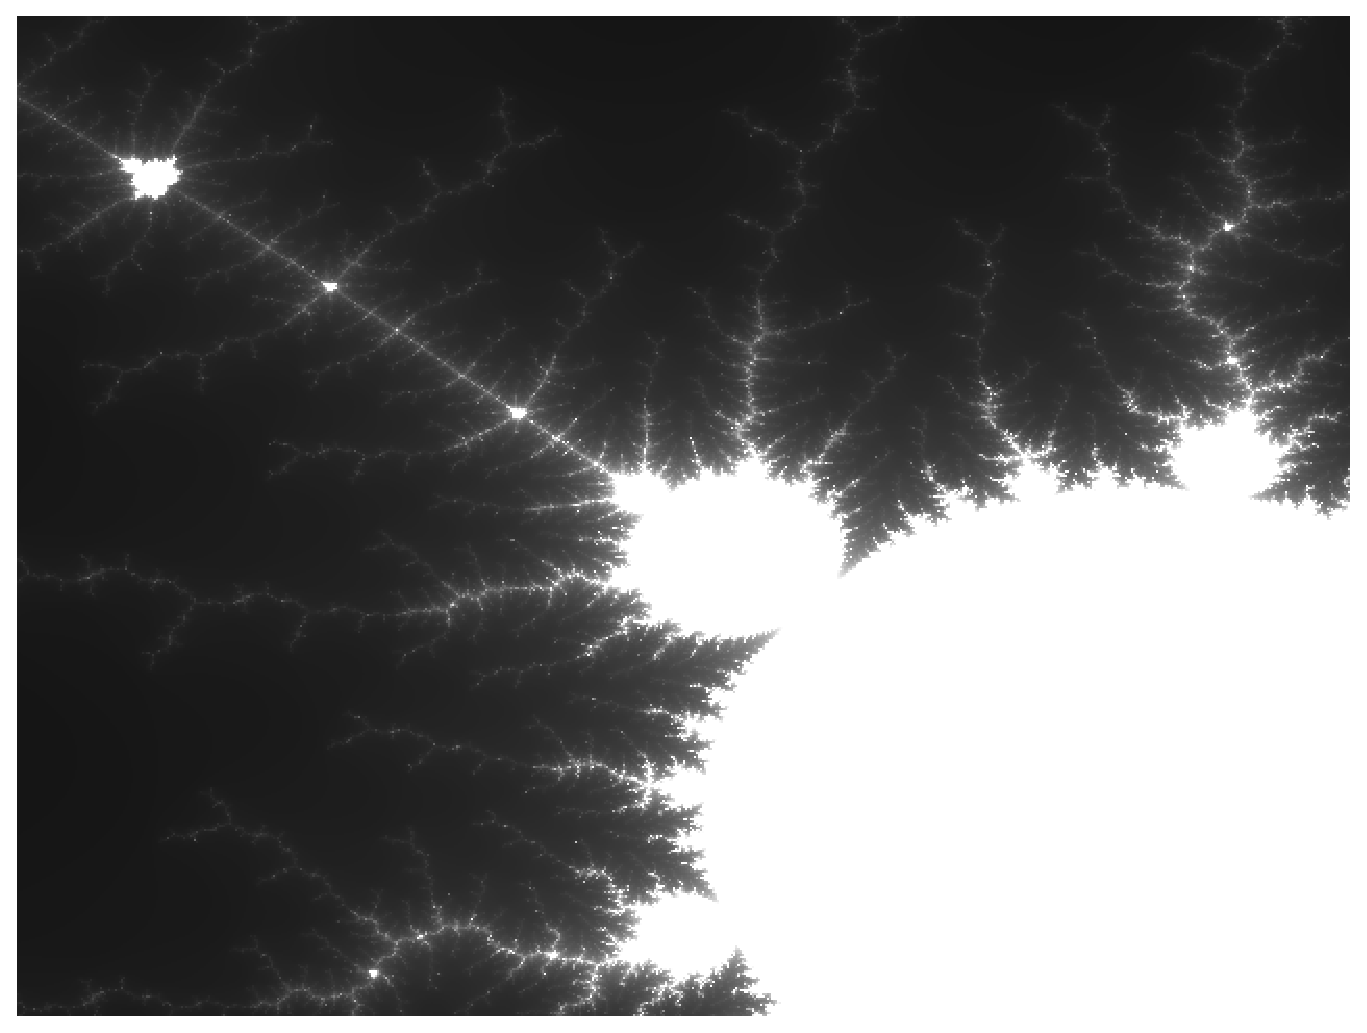
\includegraphics[width=0.7\textwidth]{images/mandelbrot_1.eps}
\caption{ Mandelbrot1 }
\label{mandelbrot_1}
\end{center}
\end{figure}

\pagebreak



\subsection{Este es el T�tulo de una Subsecci�n}

Texto de la subsecci�n...

\begin{lstlisting}[
    language=bash,
    basicstyle=\small\ttfamily
]
    $ ./tp0 --width 0.00913463304208467 --height 0.00913463304208467
            --center -0.027010582808902495+0.7093001367538602i
            --resolution 14x11 -output -

    P2
    14
    11
    255
    255 255 255 255 255 255 107  84  88  52  39  36  39  64 
    255 255 255 255 255 255  86 125  61  47  40  39  66  52 
    255 255 255 255 255 255 255  63  59  64  42  42  44  63 
    255 255 255 255 255 255 228 255 230  53  45  44  45  46 
    255 255 255 255 255 255 255 202 140  54 110  85  49  52 
    255 255 255 255 255 255 255 179  74  61  58  64  81  90 
    255 255 255 224 255 255 164 139 105  85 100 196 105 117 
    255 149 217 144  73 230 158  71 154 175  92  75  62  49 
    255  90  78  58  53  56  81  58  81  74  97  93 115  61 
    194 255 255 118  48  43  45  49  70  66  97  83  49  55 
     58  64  84  72  47  48  38  55  52  45  43 123  38  34 

\end{lstlisting}

\begin{figure}[!htp]
\begin{center}

\includegraphics[width=0.7\textwidth]{images/mandelbrot_2.eps}
\caption{ Mandelbrot2 }
\label{mandelbrot_2}
\end{center}
\end{figure}

\pagebreak

\section{Codigo Fuente}

Texto de la seccion...

\subsection{main.c}
\begin{lstlisting}[
    language=c,
    basicstyle=\small\ttfamily
]


\end{lstlisting}

\subsection{default\_values.c}
\begin{lstlisting}[
    language=c,
    basicstyle=\small\ttfamily
]

\end{lstlisting}
\pagebreak


\subsection{parse\_opt.c}
\begin{lstlisting}[
    language=c,
    basicstyle=\small\ttfamily
]


\end{lstlisting}
\pagebreak

\subsection{mandelbrot.c}

\begin{lstlisting}[
    language=c,
    basicstyle=\small\ttfamily
]

\end{lstlisting}
\pagebreak



\section{Pruebas}

El desarrollo y validacion del desarrollo se baso en un set de pruebas unitarias.
Como framework de unittesting elegimos CuTest, debido a su portabilidad y su facilidad para compilar en MIPS.

\section{Extras}

Desarrollamos un wrapper en Python

\href{http://home.facu.tk/mandelbrot}{http://home.facu.tk/mandelbrot}

\section{Repositorio}

El codigo fuente del tp, el wrapper y este documento esta alojado en github.

\href{https://github.com/facutk/66.20}{https://github.com/facutk/66.20}

\section{Conclusiones}

Se present� un modelo para que los alumnos puedan tomar como referencia en la redacci�n de sus informes de trabajos pr�cticos.


\begin{thebibliography}{99}

\bibitem{MANDEL01} Introduction to the Mandelbrot Set, http://www.ddewey.net/mandelbrot/

\bibitem{MANDEL02} Mandelbrot set, http://en.wikipedia.org/wiki/Mandelbrot_set

\bibitem{MANDELCODE} Mandelbrot C Renderer, http://rosettacode.org/wiki/Mandelbrot_set#PPM_non_interactive

\bibitem{PGM} PGM format, http://en.wikipedia.org/wiki/Netpbm_format#PGM_example

\bibitem{GETOPT} getopt_long(3), http://linux.die.net/man/3/getopt_long

\bibitem{SSCANF} sscanf(3), http://linux.die.net/man/3/sscanf

\bibitem{FWRITE} fwrite(3), http://man7.org/linux/man-pages/man3/fwrite.3.html

\bibitem{STDOUT} Standard streams, http://en.wikipedia.org/wiki/Standard_streams

\bibitem{CUTEST} CuTest: C Unit Testing Framework, http://cutest.sourceforge.net/

\bibitem{MAKE} Makefile, http://www.cs.colby.edu/maxwell/courses/tutorials/maketutor/

\bibitem{GXEMUL} GXemul, http://gxemul.sourceforge.net/

\bibitem{NETBSD} The NetBSD Project, http://www.netbsd.org/

\bibitem{SSH} Secure Shell (SSH), http://en.wikipedia.org/wiki/Secure_Shell

\bibitem{GIT} git - the simple guide, http://rogerdudler.github.io/git-guide/

\bibitem{PYTHON} Python, https://www.python.org/

\bibitem{FLASK} Flask Quickstart, http://flask.pocoo.org/docs/0.10/quickstart/

\bibitem{JQUERY} jQuery, http://jquery.com/

\bibitem{LATEX} LaTex, http://www.latex-project.org/

\end{thebibliography}

\end{document}
